\chapter{Background}\label{chapter:background}

\glsresetall

Most of the steps in this thesis utilize neural networks. Therefore, we briefly discuss what a neural network is and describe the types of neural networks that are relevant for this thesis, which include \glspl{cnn}, \glspl{gan} and \glspl{rnn}.

\section{Neural Networks}
With its original name being the \emph{multi-layer perceptron}, a neural network is a type of pattern recognizer that is somewhat similar to the human brain structure. Its main components are neurons, which are usually connected in a specific pattern to create a learnable mapping from an input vector to an output vector. Those vectors can be almost anything, like images, text, measurements or class labels.

In its original configuration, the neurons were organized in layers, with the output of one layer being the input of the next layer. The \emph{depth} of a network is then said to be the number of successive layers between the input and the output of the network.

The two biggest inventions that made neural networks successful were the inclusion of \emph{nonlinearities} and the \emph{backpropagation algorithm}.

\textbf{Nonlinearities.} In its first version, the output of a neuron was simply a linear combination of all of its inputs plus a constant bias. Or, if you combine all neurons of a layer into a single mathematical operation, the output of the layer was simply the input of the layer multiplied with a weight matrix plus a bias vector. The problem that arises is the fact that having multiple layers stacked on top of each other doesn't change the fact that the entire network can still be reduced down to a single linear operation on the input data. It therefore isn't possible to learn any function that contains a non-linearity, which includes almost any practical function.

The solution was to apply a non-linear activation function to each neuron output value. In the beginning, this function used to be the \emph{sigmoid} or \emph{tanh} function, but later studies revealed that simpler functions yield comparable or even improved results and have large performance benefits. Most modern networks use the \emph{relu} function or its variants, like the \emph{leaky relu}.

A layer of a neural network might therefore look like this:
\begin{equation}\label{eq:networklayer}
layer(\vec{x}) = relu(\vec{A} \vec{x} + \vec{b})
\end{equation}
\begin{equation}
relu(\vec{x}) = \begin{cases}x_i$,$ & $for all $ x_i > 0\\0$,$ & $for all others$\end{cases}
\end{equation}


\textbf{The backpropagation algorithm.} Most networks are trained by defining a loss function that compares the network output to the desired output, followed by minimizing the result of the loss function by modifying the network parameters. While there were already several algorithms that perform this minimum search, like the \emph{gradient descent} algorithm, most of them require the \emph{gradient} of the loss value with respect to the network weights. A network that is multiple layers deep and contains an adequate amount of neurons per layer quickly becomes very resource-intensive to train, and computing every single gradient by solving the network equation over and over again becomes impractical. This is where the backpropagation algorithm comes into play. Its main idea is to compute the gradients layer by layer, starting at the loss value. It achieves that by utilizing the decomposition of a gradient into layer-wise partial derivatives, as shown in the following example. Here, we compute the gradient of the loss $E$ for the weights $w_1$ through the network layer outputs $x_1$ and $x_2$:

\begin{equation}
\frac{\delta E}{\delta w_1} = \frac{\delta E}{\delta x_2}\frac{\delta x_2}{\delta x_1}\frac{\delta x_1}{\delta w_1}
\end{equation}

\begin{figure}
  \centering
  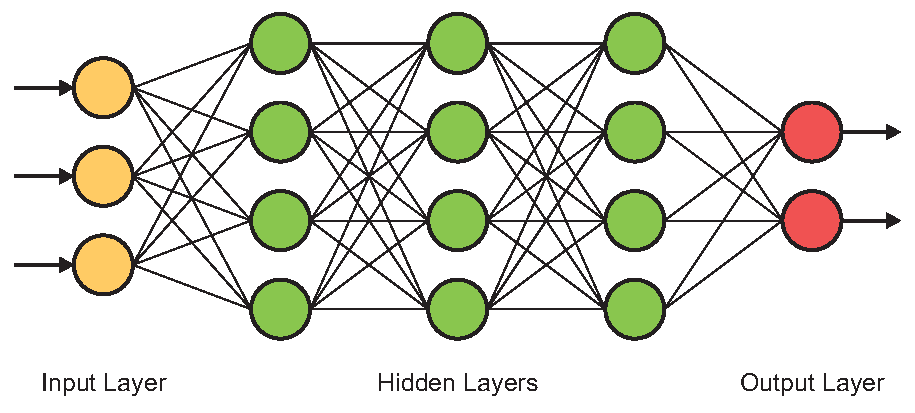
\includegraphics[width=0.8\textwidth]{../assets/background/neural_network.pdf}
  \caption[Schematic of a fully connected network]{Schematic of a fully connected network. Each neuron is connected to all neurons of the previous layer.}
  \label{fig:neuralNetwork}
\end{figure}

\textbf{Network variants.} The configuration where all neurons of one layer are being connected to all neurons of the next layer is nowadays known as a \emph{fully connected} network, as shown in \cref{fig:neuralNetwork}. It has the advantage that it can represent almost any function, but it also has major drawbacks. Most data types have invariants that this type of network does not have built-in, and it therefore needs a lot of training data to learn them explicitly. This is especially true if we deal with image data, as images are very high dimensional data with an inherent translation invariance for most recognition tasks. This lead to the development of Convolutional Neural Networks (\glspl{cnn}).

\section{Convolutional Neural Networks}
This type of network builds on the layer-wise architecture of the fully connected network, but introduces some crucial improvements for image data. Specifically, it enforces translation invariance by tying weights of different spacial locations together.

Its first step is to push the one-dimensional vector representation into a higher dimensionality. For two dimensional images, this is usually a matrix of size $(width \times height \times features)$, keeping the spacial dimensions encoded separately, and having one feature vector per spacial coordinate.

The network layer can still be represented in a matrix multiplication like \cref{eq:networklayer}, but the matrix itself now represents a convolution operation with a specific kernel. That kernel connects each output coordinate to a number of neighboring input coordinates. This means that each feature point is no longer connected to all feature points of the previous layer, but only to those that are spacially relevant for it. Further, every feature point of one layer is computed with the same kernel, only the position of the kernel is adjusted for each point. 

Combining multiple convolution layers has the effect of combining low-level features to higher level, more complex features. To visualize that, the first layer might detect line segments of different directions, the second layer might combine those to patterns like curves, checkerboard patterns or gradients, the third layer might combine those to more complex shapes like eyelashes or teeth, the fourth one might combine those to eyes, mouth or ears, and the fifth layer could then be a face detector. An example for such a \gls{cnn} can be seen in \cref{fig:cnn}.

In most cases, convolution layers are followed by a subsampling, which causes the information to become more and more global from layer to layer, so that the final layer usually only consists of a single feature vector with no spacial information. This loss of locality is mitigated by giving deeper layers increasingly more feature depth, effectively shifting the information from a spacial to a global representation. In some cases, the convolutional network is followed by a fully connected network for further processing.

Tying features together in a shared kernel reduces the dimensionality of the network drastically while preserving the ability to robustly detect and process almost any humanly distinguishable image content. Nonetheless, training \glspl{cnn} is still a demanding task, which caused the development to stall until the computing performance finally caught up in recent years.

\begin{figure}
  \centering
  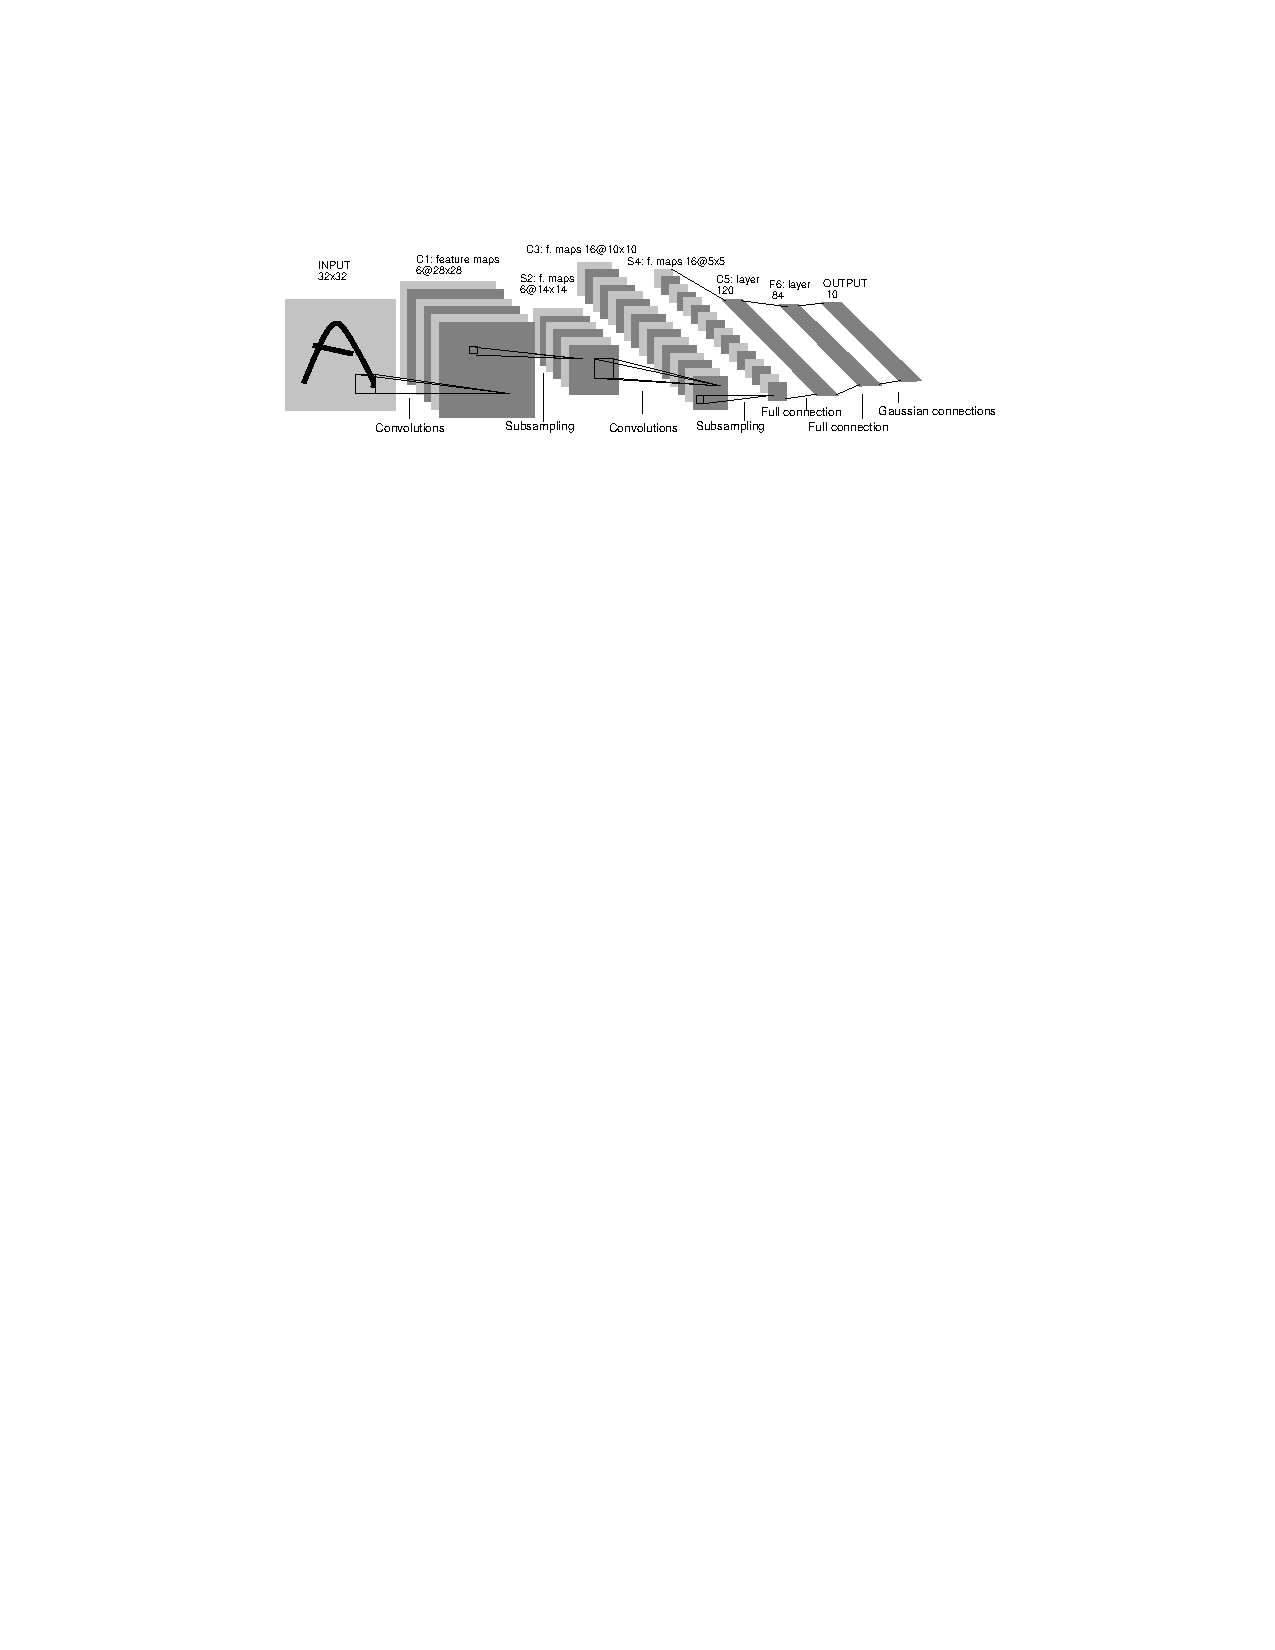
\includegraphics[width=0.9\textwidth]{../assets/background/cnn.pdf}
  \caption[Example of a \gls{cnn} architecture]{Example of a \gls{cnn} architecture. This network, called \emph{LeNet-5}, is a \gls{cnn} with two convolution layers with subsampling, followed by fully connected layers. Its purpose is to detect digits. Source:~\cite{cnn}}
  \label{fig:cnn}
\end{figure}


\section{Generative Adversarial Networks}
Contrary to \glspl{cnn}, \glspl{gan} don't actually describe a specific network layout, but instead refer to a new training method for existing networks. This mainly consists of replacing or extending the existing loss function with another network that learns the loss during training. Especially in image generation, most loss functions used to be based on the \gls{mse} between generated and real training images. This technique has major drawbacks, as a simple thought experiment shows. Imagine a task where the goal is to produce red and green squares: A network trained with an \gls{mse} loss would always produce yellow squares, because on average, this is always the best guess. However, if we replace the loss with another network that tries to find the differences between real and generated images, it will immediately pick up on the fact that yellow squares strongly indicate generated images. This in turn forces the generating network to produce either red or green squares. Those two networks are called \emph{generator} and \emph{discriminator}. The \emph{generator} network ($G$) generates the output data and the \emph{discriminator} network ($D$) tries to find the difference between the real and the generated data.

The entire training process can then be expressed by a min-max game between the generator and the discriminator, where $d_{real}$ is the training data, consisting of pairs of real inputs and outputs. The goal is that the network learns a mapping function between them. The game would then look like this:

\begin{equation}\label{equation:minMaxGame}
\min_D\max_G \sum_{\vec{x}, \vec{y} \in d_{real}} \norm{1 - D(\vec{y})} + \norm{D(G(\vec{x}))}
\end{equation}

This means that the discriminator gets rewarded for outputting a value close to $1$ for real images and a value close to $0$ for generated images, in the attempt to minimize this entire term. The generator, however, gets rewarded for preventing the discriminator from doing so, by generating images that are indistinguishable for the discriminator.
This game reaches its equilibrium point when there is no noticeable difference between the generated and real images any more, allowing for a very high-quality output of the network.

While \cref{equation:minMaxGame} is not the original mathematical representation, it is the most commonly used version, as it cannot saturate easily.


\begin{figure}
  \centering
  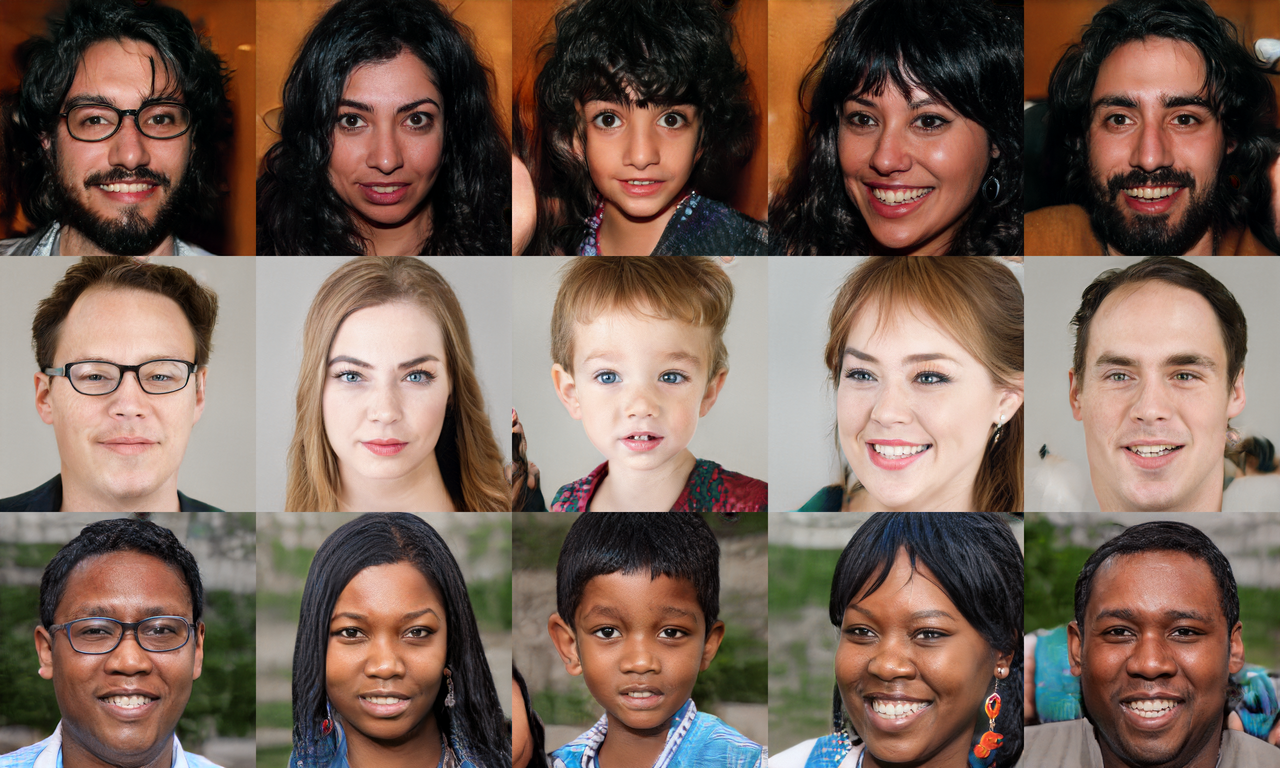
\includegraphics[width=0.75\textwidth]{../assets/background/stylegan-teaser.png}
  \caption[Photorealistic human faces generated by a \gls{gan}]{Photorealistic human faces generated by a \gls{gan}. Source:~\cite{styleGan}}
  \label{fig:ganFaces}
\end{figure}

A very good demonstration of the effectiveness of this approach is the generation of human faces, as shown in \cref{fig:ganFaces}.

\section{Recurrent Neural Networks}

So far, all neural networks we talked about were uni-directional, meaning they had one defined input and one defined output, and all connections were directed towards that output. This is insufficient for many problems that do not have a fixed input or output size, but rather a variably sized stream of data, like video or audio samples.

The state-of-the-art solution for those problems are \emph{Recurrent Neural Networks} (\glspl{rnn}). Recurrent networks also have an input and output vector, but they also have an additional connection to the next and previous timestep. This enables them to \emph{memorize} information and therefore to process data with long term temporal dependencies.


\begin{figure}
  \centering
  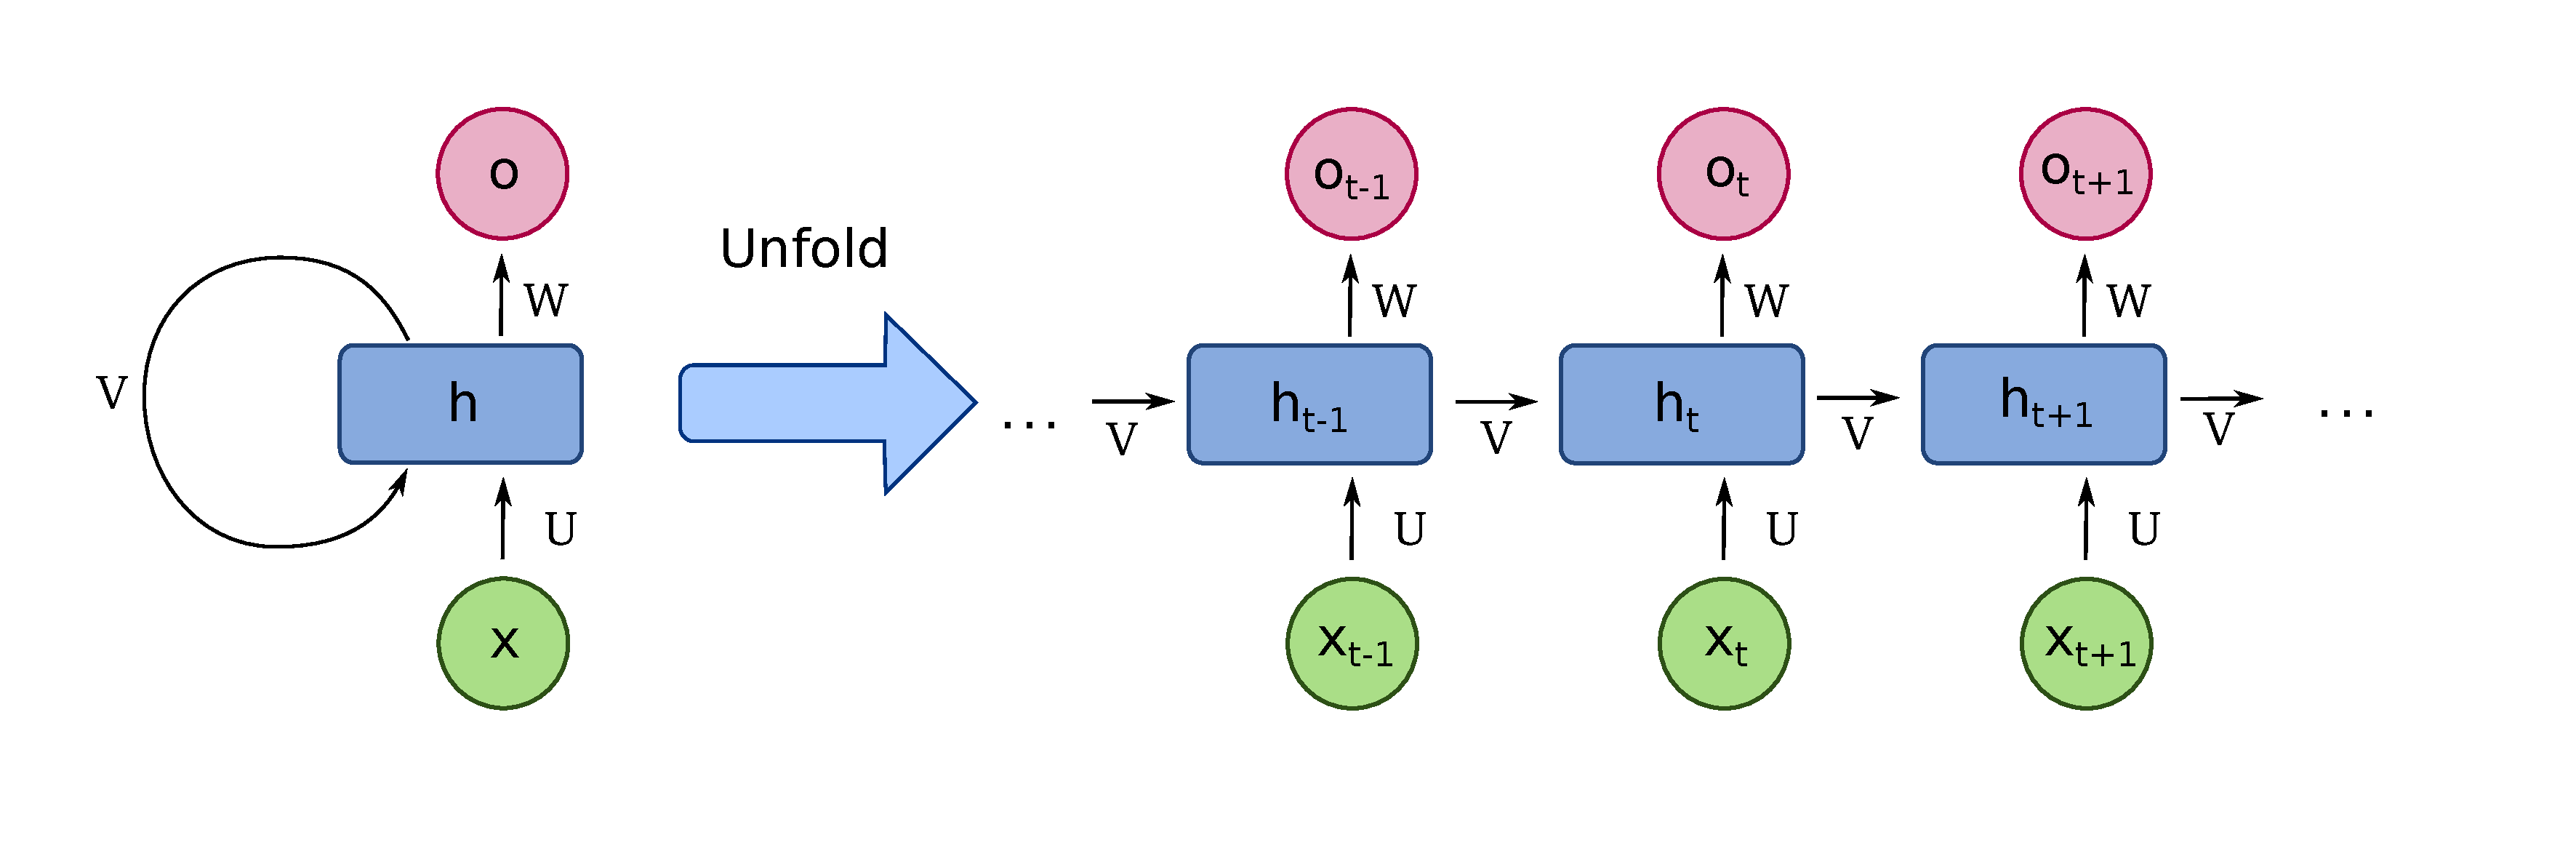
\includegraphics[width=0.9\textwidth]{../assets/background/Recurrent_neural_network_unfold.pdf}
  \caption[Schematic of an \gls{rnn}]{Schematic of an \gls{rnn}. The left side shows a compressed version, the right side shows an unfolded version. $x$ is the network input, $h$ is the hidden state and $o$ is the network output. $U$, $V$ and $W$ are the weights of the network, in many cases themselves being fully connected neural networks. Note that $V$ is the recurrent connection, which feeds data from one time step to the next. Source:~\cite{rnnWikipedia}}
  \label{fig:rnn}
\end{figure}

It was quickly discovered that passing information to the next time step through a simple side connection is not sufficient, as backpropagation through a big number of time steps causes the gradient to vanish, effectively preventing the network from learning long term dependencies. This problem was overcome by adding \gls{lstm} cells, which give the network the ability to decide by itself how long information should be stored. This is achieved by adding \emph{gates} to the memory connections with which the network itself can decide whether information should be kept or overwritten. This enables the gradients during the learning phase to effectively skip time steps, preventing them from vanishing.

\begin{figure}
  \centering
  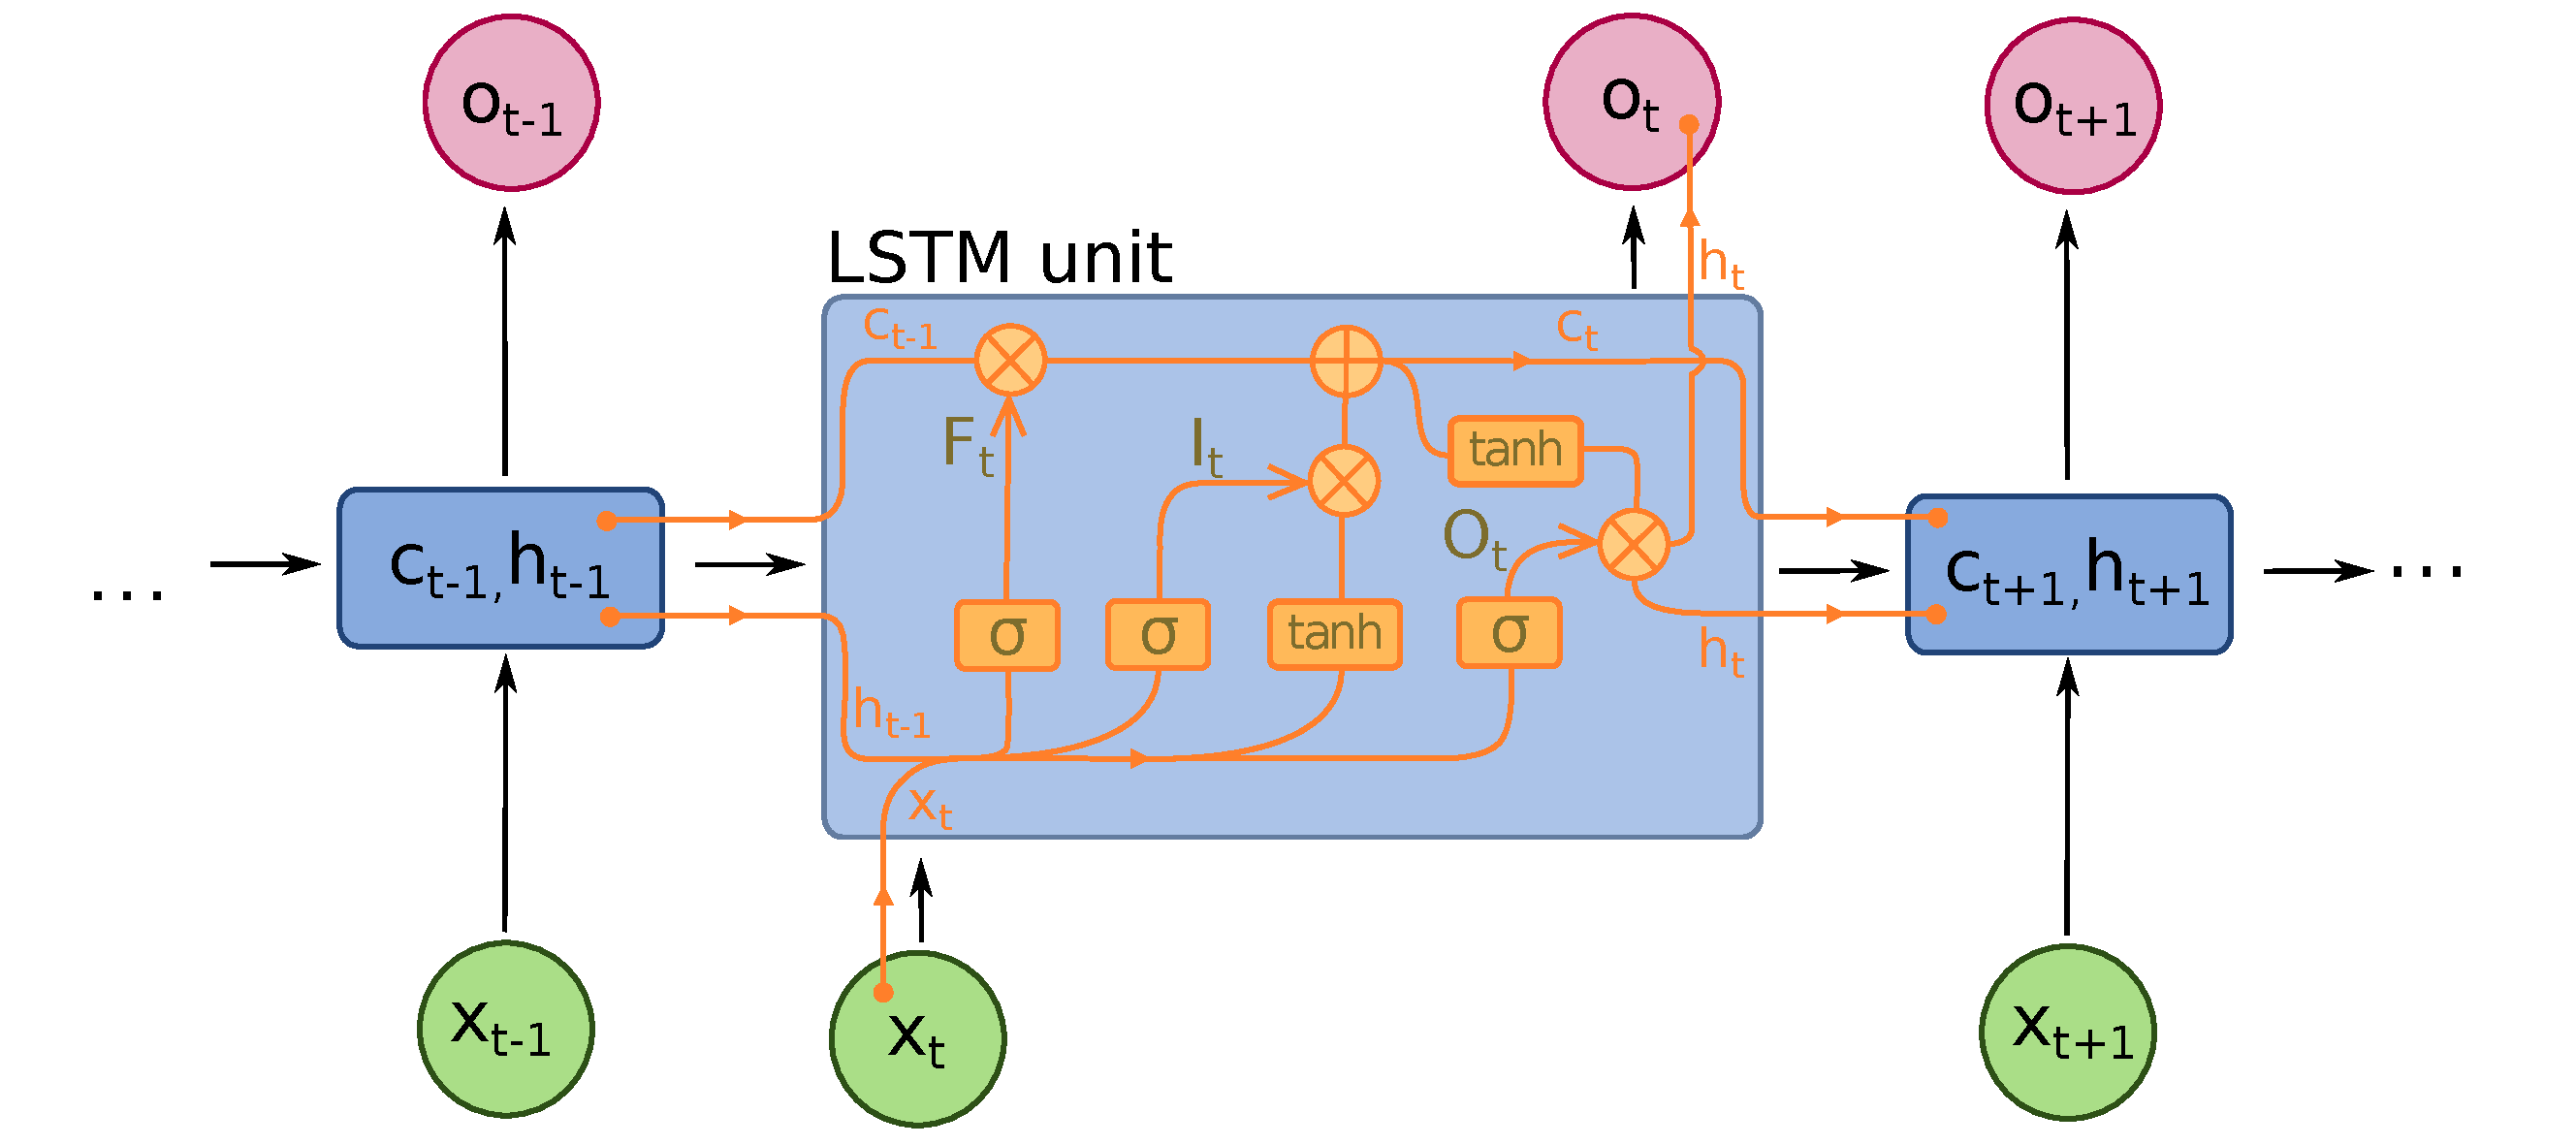
\includegraphics[width=0.9\textwidth]{../assets/background/Long_Short-Term_Memory.pdf}
  \caption[Schematic of an \gls{lstm} cell]{Schematic of an \gls{lstm} cell. Note the $\bigotimes$ symbols, which represent the gates that decide whether the cell passes on its stored information to the next timestep or replaces it with new information. Source:~\cite{rnnWikipedia}}
  \label{fig:lstm}
\end{figure}

At the time of writing, \gls{lstm} networks are state-of-the-art for most problems that require \glspl{rnn}.


